\section{Theoretical Analysis}
\label{sec:analysis}

In this section, the circuit shown in \textbf{Figure~\ref{fig:diagram_t3}} is analysed
theoretically.
\begin{figure}[H] \centering
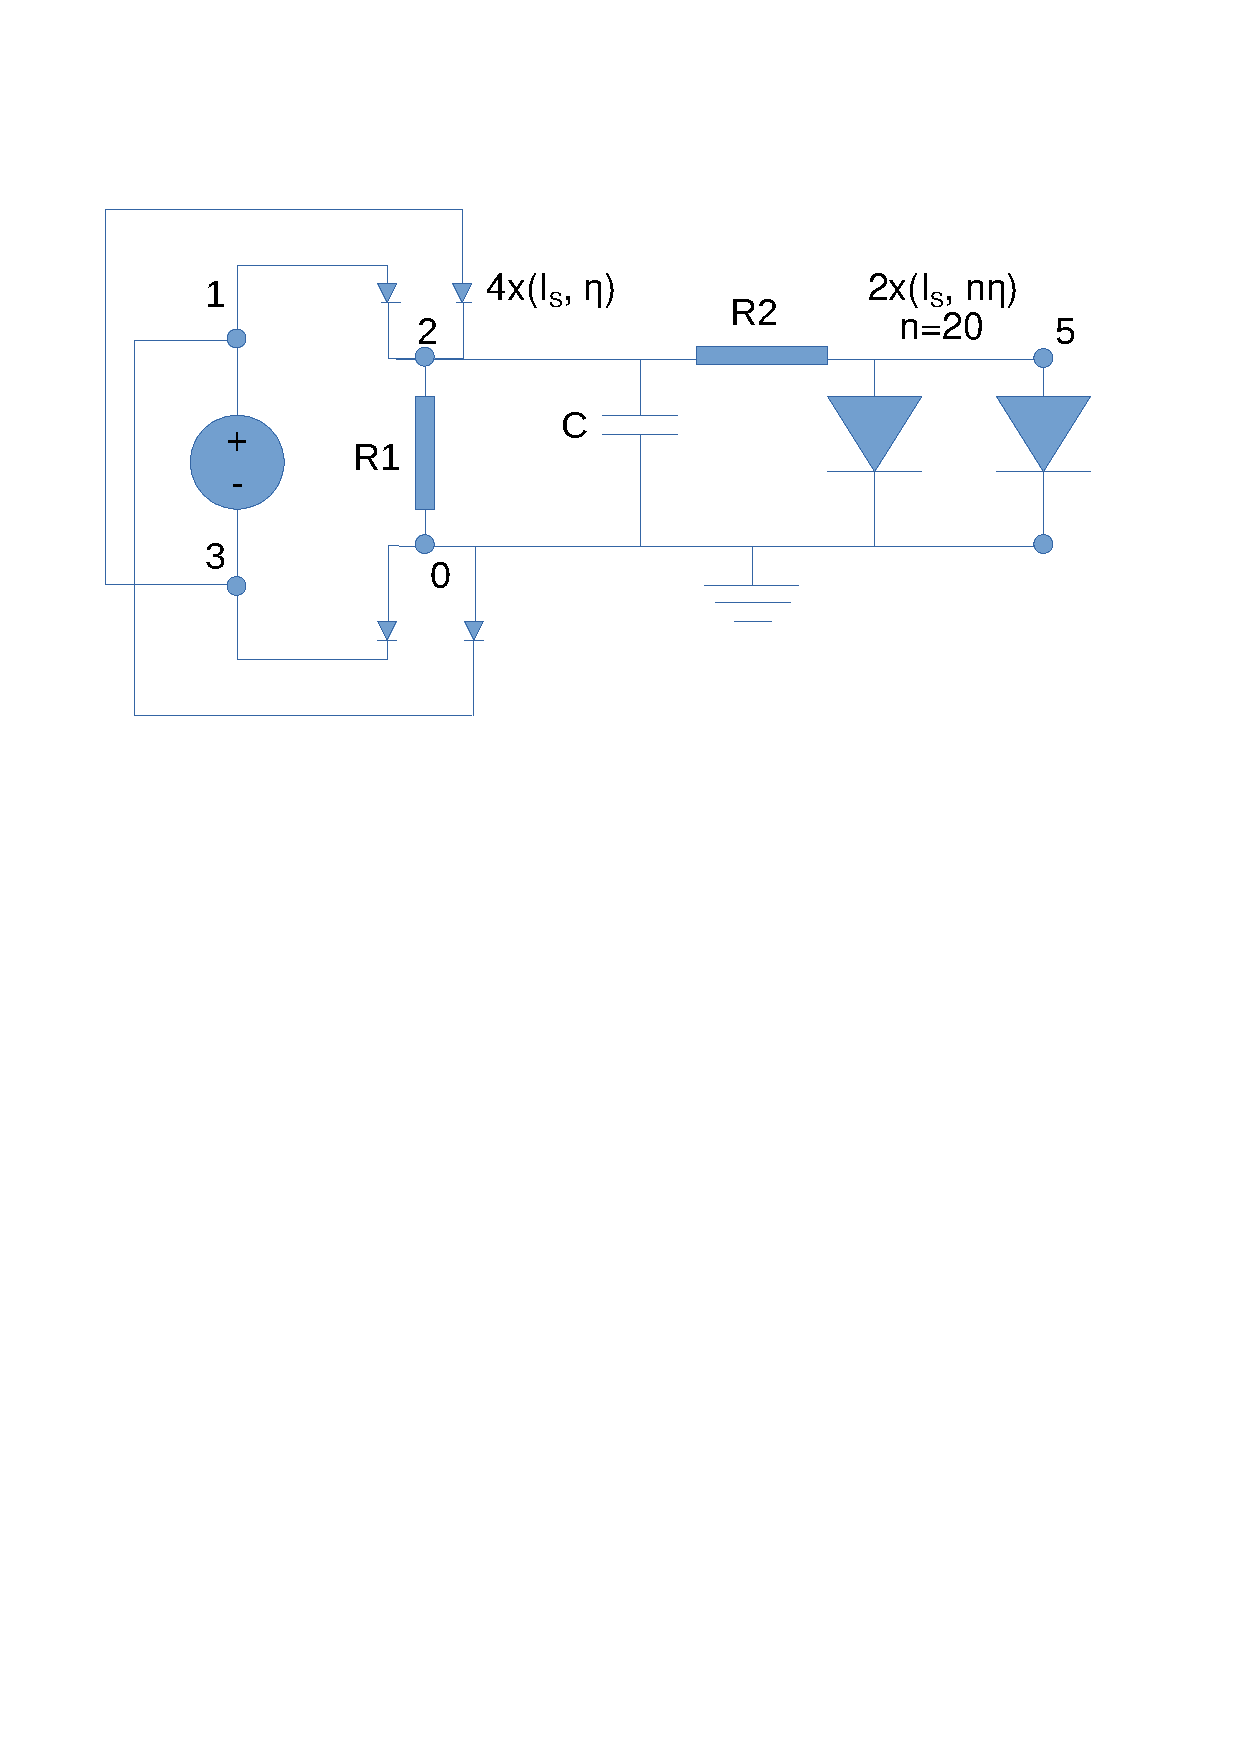
\includegraphics[width=0.5\linewidth]{diagram_t3.pdf}
\vspace{-6cm}
\caption{Diagram of the circuit considered for the computations and simulations.}
\label{fig:diagram_t3}
\end{figure}

The transformer used has an n:1 ratio. This means that the initial voltage source will have its Amplitude (A) divided by a factor of n. Therefore we can represent the voltage at the terminals of the transformer as a voltage source with an Amplitude of A/n and with the same frequency as the initial source. As noted in the previous section, this paremeter n is indeed a rational number - we considered any combination of transformer coils to be possible.

The output of the transformer will be the input of our Envelope detector. The Envelope Detector circuit is made up of a rectifier and a capacitor. The rectifier is a full-wave bridge rectifier circuit and is composed of 4 diodes and a resistor. The full-wave rectifier was used as oposed to a half-wave rectifier because the full-wave rectifier allows us to reduce the ripple without increasing the time constant, which will avoid a big raise in costs. The full-wave rectifier reduces the ripple because the voltage that comes out of the transformer will leave the rectifier oscillating at twice the frequency, which helps us in our ripple problem, by reducing the period corresponding to the wave ripple.

The output of the Envelope Detector will be the input of the Voltage Regulator. The voltage regulator is made up of 42 diodes, two series of twenty diodes in parallel (as this proved to be an inexpensive way to reduce by half the equivalent incremental resistance of the regulator's diodes, and thus minimize ripple even more) and one resistance. The resistance is in series with the paralel of 2 rows of 21 diodes each. The diodes in each row are in series. The output of the paralel of diodes is the output of the AC/DC converter.

In the Envolope Detector the diode model used has an ideal diode and a voltage source while in the Voltage Regulator de Diode model has an ideal diode, a voltage source and a resistor. Do note that the voltage Von for this diode model was obtained by dividing the the output voltage of the Ngspice simulation by the number of diodes in series, in order to achieve a more realistic model for the theoretical analysis. This yielded Von = 0.5714 V, a slight deviation from the standard Von = 0.7 V generally used.

The ratio of the transformer and the values of the resistors, the capacitor and nº of diodes are presented in the following table, along with a side-by-side comparison of the corresponding results (ripple, average, merit) in the theoretical analysis (right) and the Ngspice simulation (left).

\hfill
 \parbox{1\linewidth}{
  \centering
  \begin{tabular}{|l|l|l|r|}
    \hline    
    {\bf Parameter} & {\bf Simulation} & {\bf Theoretical } & {\bf Units }\\ \hline
    Zi & 766.402 & 640.49 & Ohm\\ \hline
Zo & 4.49605 & 2.9364 & Ohm\\ \hline
Cost & 8116 & Cost & MU\\ \hline
uco & 3106933.000 & 2123123123123.000 & Hz\\ \hline
lco & 7.924 & 2123123123123.000 & Hz\\ \hline
Bandwidth & 3106925.076 & 2123123123123.000 & Hz\\ \hline
Gainv(out) & 56.041 & -107.220 & [adimensional]\\ \hline
MERIT & 2707.5316 & -104.2260 & gold medals\\ \hline

  \end{tabular}
  \label{tab:results}
    %\caption{Side-by-side comparison of the circuit parameters (resistors, capacitors, etc) and the corresponding results (ripple, average, merit)}
    

  }


    The only difference is in the ripple value, given the Von parameter for the thoeretical model was derived from the simulation results - this accounts for the perfect fit between the simulated and predicted average output voltages. As such, the merit figures differ given the ripple value is found in denominator - this means that, despite the ripple deviation being in the order of microvolts, this deviation is amplified in the merit formula. In adition, the precision of octave and ngspice floating point is different, which may account for part of the differences found. But more importantly, the difference obtained was mainly due to the fact that the models
used for the diodes in the theorethical analysis differ from those used by Ngspice. The diode
model used by Ngspice is way more complex than the one implemented theoretically.
  
  The next figures present the plots required, resulting solely from the theoretical analysis.

%In \textbf{Table~\ref{tab:theoretical}} the values for the branch currents and the node voltages obtained from the Octave script for both methods are presented. Here, the node voltages in the mesh method were computed from the respective currents, which were determined as described in the previous subsection.



\subsection{Output of the voltage regulator circuit, compared with the output sinusoidal voltage of the transformer and the envelope detector voltage}

\par
\begin{figure}[H] \centering
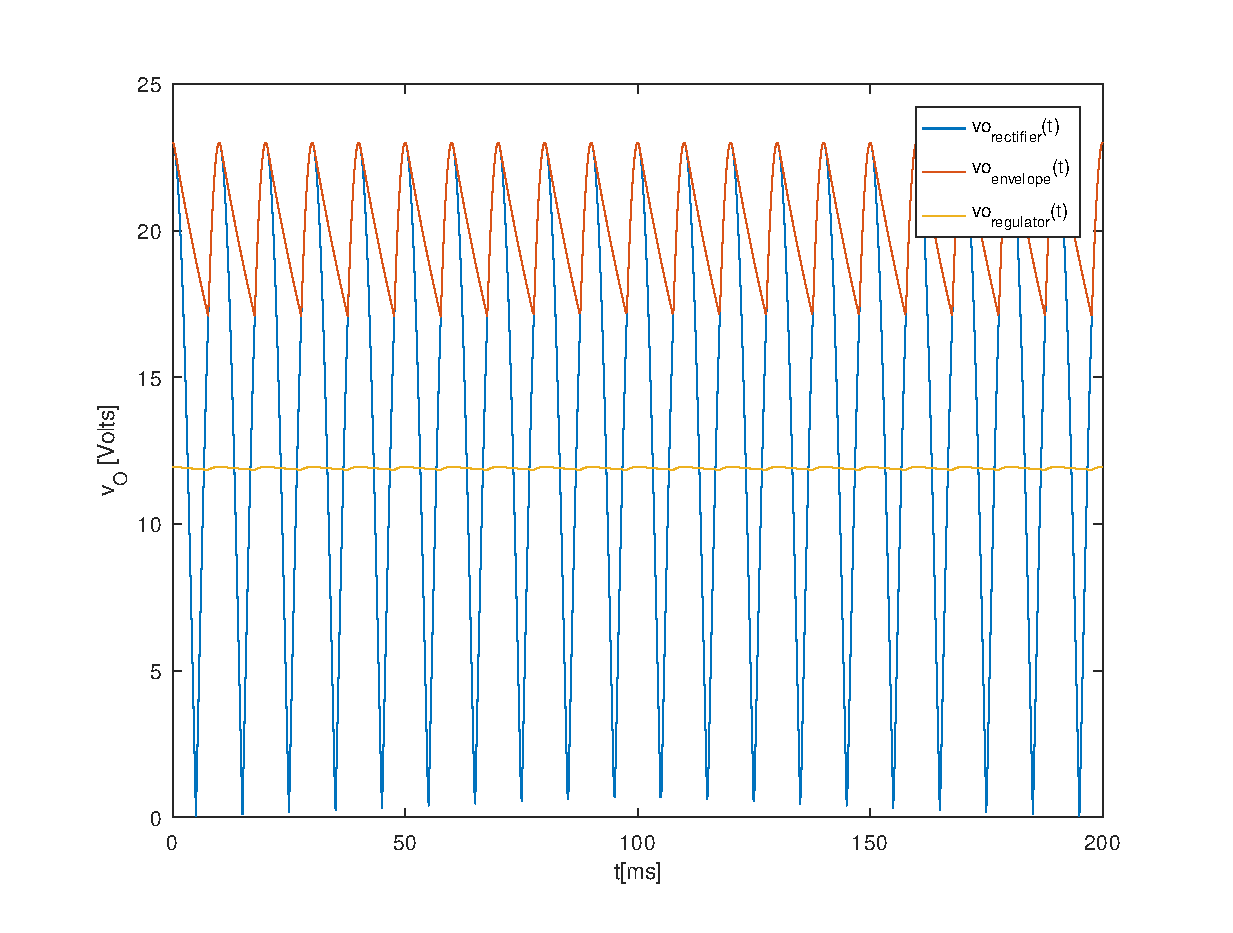
\includegraphics[width=0.6\linewidth]{all_vout.eps}
\caption{Output of the voltage regulator circuit (yellow), compared with the output sinusoidal voltage of the transformer (blue) and the envelope detector voltage (red)}
\label{fig:all_vout}
\end{figure}


\subsection{Output of the Envelope Detector (acting on the output of the full-wave rectifier)}

\par
\begin{figure}[H] \centering
\includegraphics[width=0.6\linewidth]{envelope.eps}
\caption{Output of the Envelope Detector (acting on the output of the full-wave rectifier)}
\label{fig:envelope}
\end{figure}



\par
\begin{figure}[H] \centering
\includegraphics[width=0.6\linewidth]{regulator.eps}
\caption{Output of the voltage regulator circuit, so as to visualize the ripple effect in greater detail}
\label{fig:regulator}
\end{figure}

\par
\begin{figure}[H] \centering
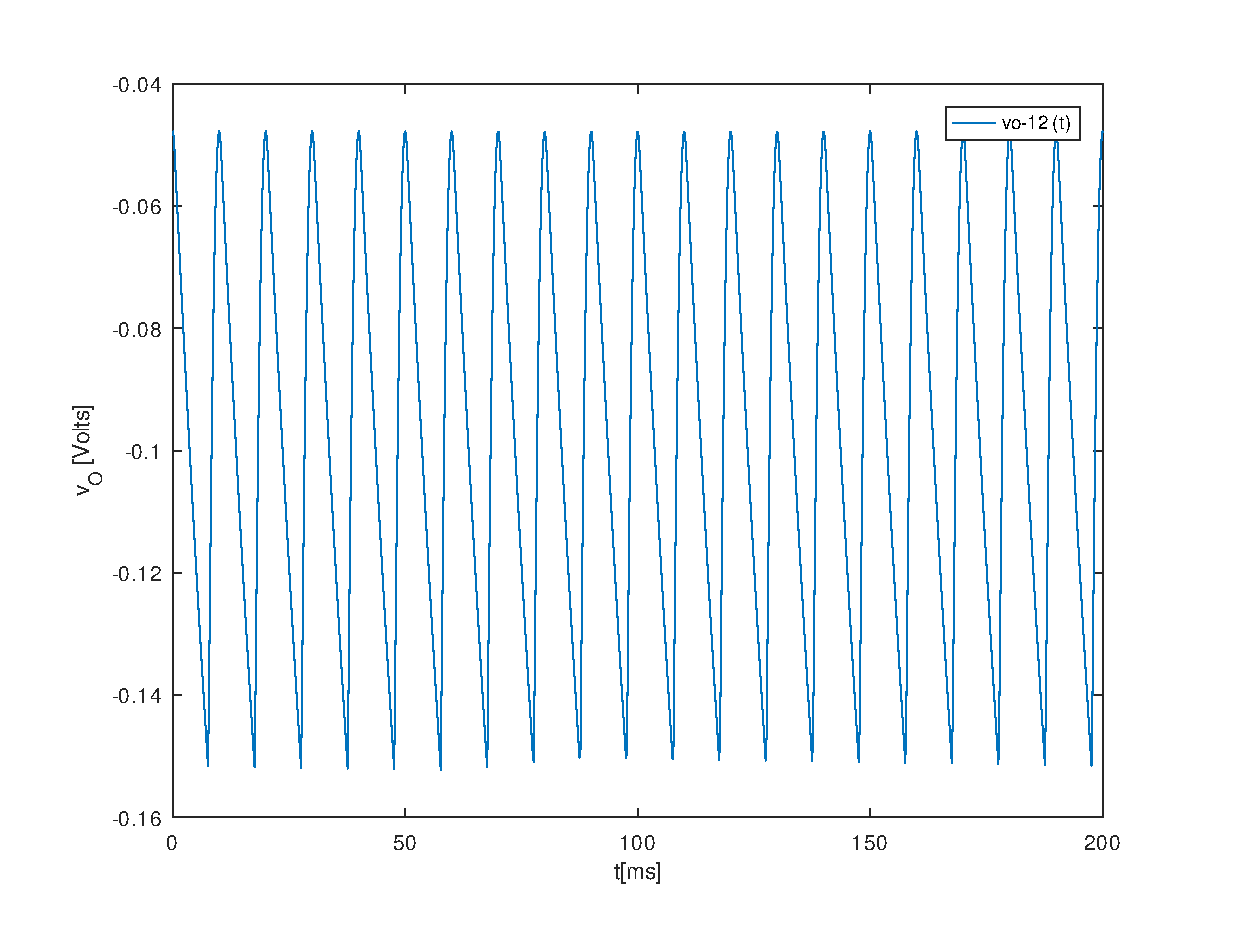
\includegraphics[width=0.6\linewidth]{deviation.eps}
\caption{($v_O$ – 12) (output AC component + DC deviation)}
\label{fig:deviation}
\end{figure}


%\begin{figure}[H] \centering
%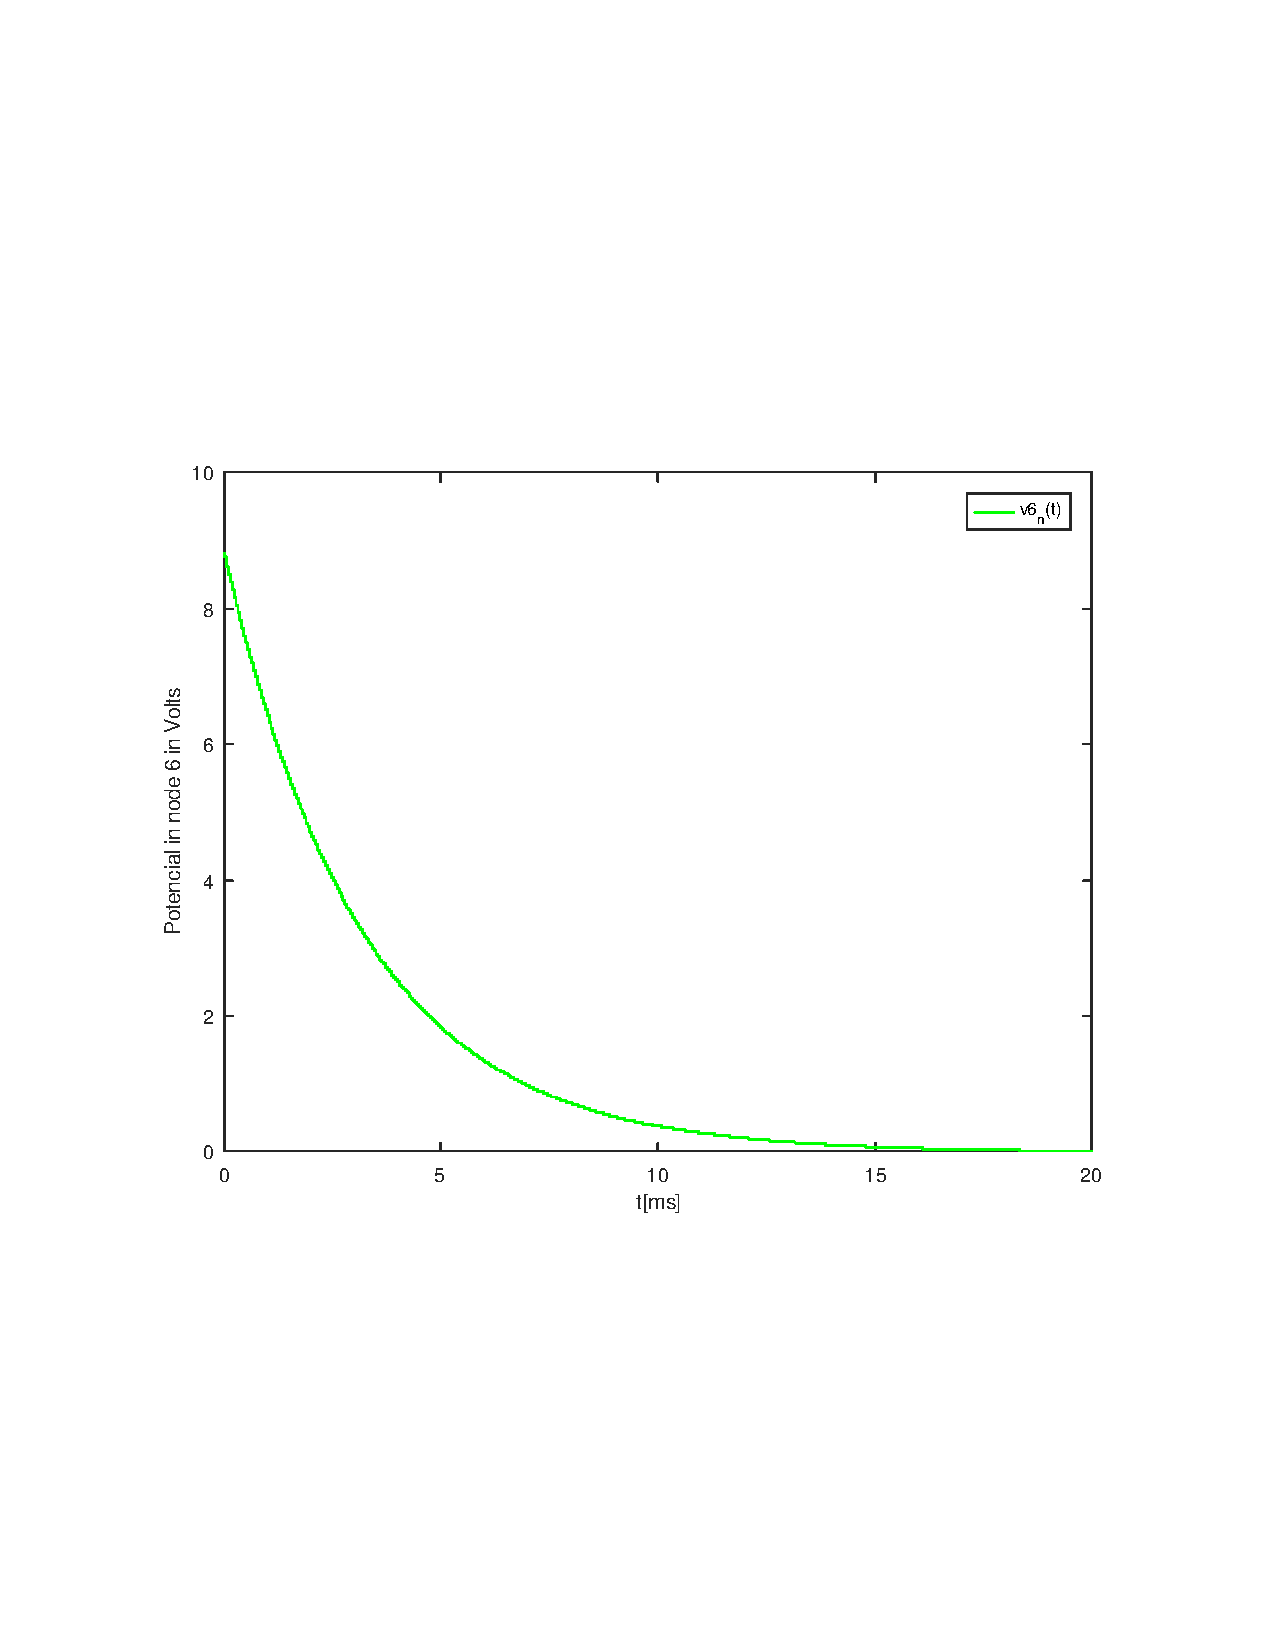
\includegraphics[width=0.9\linewidth]{natural_tab.pdf}
%\caption{Natural response of $V_6$ as a function os time in the interval from [0,20] ms}
%\label{fig:natural}
%\end{figure} 



%\begin{figure}[H] \centering
%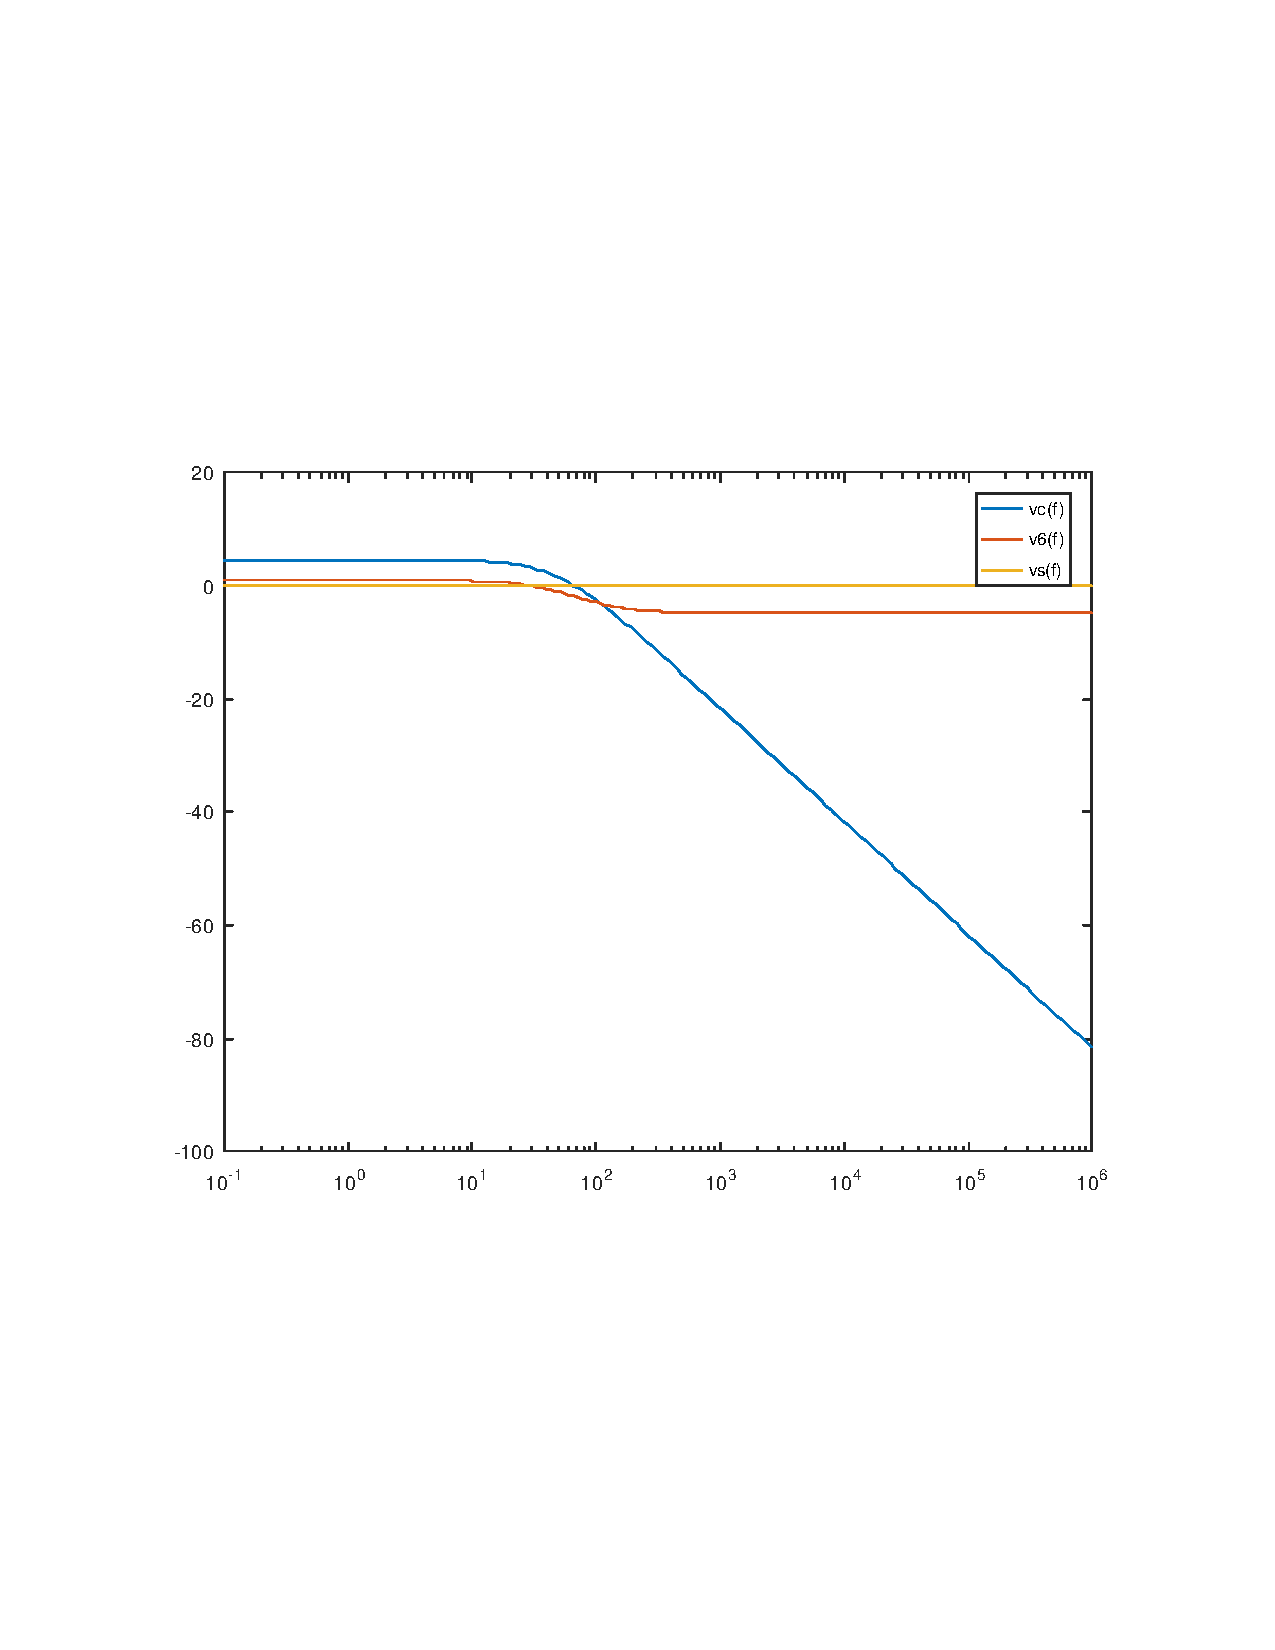
\includegraphics[width=0.9\linewidth]{freq_resp_tab.pdf}
%\caption{Graph for amplitude frequency response, in dB, of $V_c$, $V_6$ and $V_s$ for frequencies ranging from 0.1Hz to 1MHz (logarithmic scale).}
%\label{fig:freq_resp}
%\end{figure}




\pagebreak


